% ===========================================================================
% v3 §7 — THE OBJECT-AND-ACTION MODEL (NEW; ~1 pp; figure F5)
% Draft r2 (2026-09-03): numbers-verifier fixes — ten schemas = nine object types + the approvals file; quarantine
% writes a manifest; invalidate records which step changed.
% Draft r1 (2026-09-03), architecture block with §3 r4 and §4 (decision 20: one gate for §3+§4+§7).
% Tone per decision 18: describe what is typed and linked on disk and which actions are first-class;
% PROPOSED parts named once, no defect chronicle. Decision 19: description of a design, no claims.
% Census: working tree 2026-09-02, tracked code 4df6884; schemas dev/schemas/ (10); roster rows 18–24.
% Figure F5 = paper_agentic/figures/fig_F5_object_action_model (gated; shas in figures/GATE_LEDGER.md).
% The ontology and provenance citations (Gruber 1993; W3C PROV-DM) enter only after their PDFs are local
% (notes/RELATED_WORK_candidates_20260903.md); the text below stands without them.
% ===========================================================================
\section{The Object-and-Action Model} \label{sec:objects}

A long campaign accumulates objects: selections, block tables, fit tables,
panels, reports, and the records about them. The harness of
\S\ref{sec:harness} works only if those objects are typed, if the links
between them are declared rather than remembered, and if the operations
that change them leave a record. Figure~\ref{fig:objects} draws the model
as it exists on disk, in four parts: the objects, the links between them,
the actions that create or change them, and the roles allowed to act.

\begin{figure*}[t]
\centering
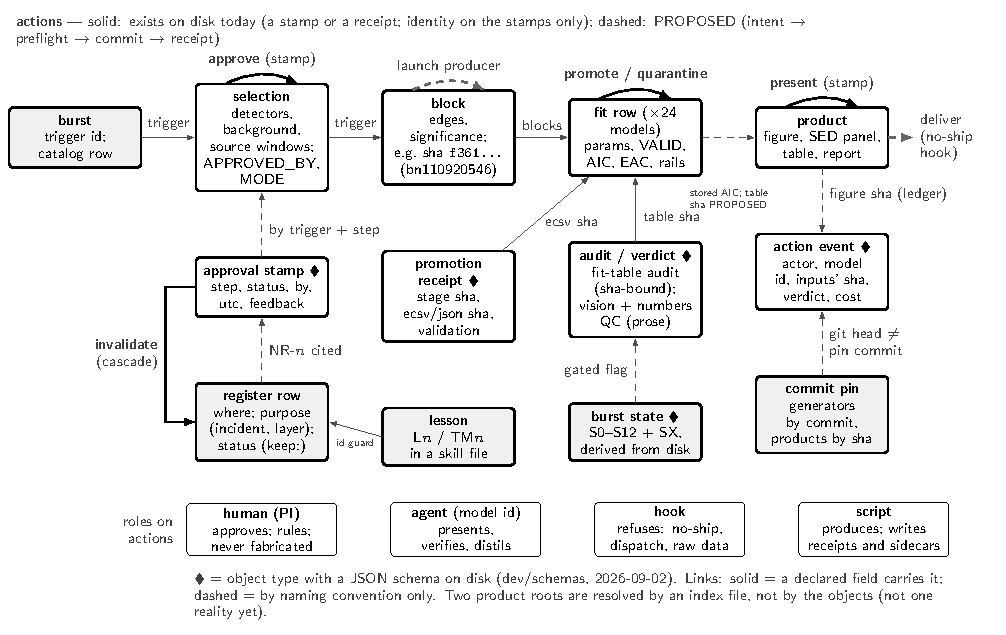
\includegraphics[width=\textwidth]{figures/fig_F5_object_action_model.pdf}
\caption{The object-and-action model. Top row: the burst's chain of
products, from trigger to report. Middle row: the records about those
products. Bottom row: the law that governs them. A diamond marks an object
type with a JSON schema on disk. Links are solid where a declared field
carries them (a trigger key, a content hash, a commit) and dashed where they
hold by naming convention. Actions are labelled arrows, solid where they
are first-class on disk today and dashed where proposed. The band beneath
names the four roles that act. Every box maps to rows of
Table~\ref{tab:roster}.}
\label{fig:objects}
\end{figure*}

\paragraph{Objects.} Thirteen object types are drawn. Five form the
burst's own chain: the \emph{burst} (trigger identifier and catalog row),
the \emph{selection} (detectors, background and source windows, with the
approver and mode stamped on it), the \emph{block table} (bin edges and
significances), the \emph{fit row} (one per model per bin: parameters,
validity flag, information criteria, effective-area corrections, rail
diagnostics), and the \emph{product} (figure, spectral-energy panel, table,
or report). Four are records about products: the \emph{approval stamp}
(step, status, approver, time, feedback), the \emph{promotion receipt}
(hashes of the staged and promoted tables and the validation that passed),
the \emph{audit or verdict} (the fit-table audit bound to the table's hash;
the vision and numbers verdicts), and the \emph{action event} (actor, model
identity, input hashes, verdict, cost). Three are the law: the
\emph{register row} (where a guard lives, the incident that bore it, its
status and keep-condition), the \emph{lesson} (a numbered entry in a skill
file), and the \emph{burst state} (one of the fourteen states of
\S\ref{sec:loop}, derived from disk), together with the \emph{commit pin}
that fixes generators by commit and products by hash. Ten JSON
schemas\prov{} cover nine object types and the per-burst approvals file
that holds the stamps; five of the thirteen drawn here are among them (the
stamp, the receipt, the audit, the action event, and the burst state), and
the others are the literature-harvest manifest and its paper records, the
frozen prediction record of \S\ref{sec:doctrine}, and the fit sidecar. The test suite validates every
instance on disk against its schema. Schemas came late: the pipeline had written
these objects for months before their shape was declared, and the first
validation pass found four spellings of one key in the literature-harvest
manifests. A schema written before the first instance would have cost less.

\paragraph{Links.} A link is declared when a field of one object names
another: the trigger key that ties a selection to its burst and a block
table to its selection; the block indices that tie fit rows to blocks; the
table hash that ties a receipt and an audit to the fit table they certify;
the lesson identifier that a register row cites, guarded by a test that
refuses duplicate identifiers. Links that hold only by convention are drawn
dashed: a stamp finds its selection by trigger and step number, a product
finds its fit rows through the stored information criteria rather than a
recorded hash, a burst state points to the verdicts it summarises by a
flag, and the commit pin relates to the action trace only through the git
head each event records. The distinction matters operationally. A declared
link can be checked by code; a conventional link can only be checked by a
reader who knows the convention. Declaring the remaining links, chiefly the
fit-table hash on every product, is the smallest step that would let the
report-conformance gate of Table~\ref{tab:roster} be written as code.

\paragraph{Actions.} An action is an operation that changes what the
campaign may claim. Four are first-class on disk today, each leaving a
typed record with an identity: \emph{approve} writes a stamp; \emph{present}
writes a stamp; \emph{promote} writes a receipt and \emph{quarantine} a manifest; and
\emph{invalidate} demotes the approvals downstream of an amended step and
records which step changed. Two are proposed and drawn dashed. \emph{Launch producer}
would wrap every pipeline run as intent, preflight, commit, and receipt,
so that a producer could not start without the plan and could not finish
without the sidecar; today the dispatch hook of \S\ref{sec:boundaries}
enforces the first half for the transitions it covers. \emph{Deliver} would
record every artifact handed to the human; today the no-ship hook refuses
an unverified figure but writes no record of what it allowed. The action
trace that would hold all six is on disk with its schema, appended by
protocol; automatic capture of every tool call is the boundary item listed
in Table~\ref{tab:roster}.

\paragraph{Roles.} Four kinds of actor appear on actions, and the model
fixes what each may do. The \emph{human} approves and rules, and no
approval is ever written on the human's behalf. The \emph{agent}, stamped
with its model identity, presents, verifies, and distils. The \emph{hook}
refuses. The \emph{script} produces and writes its receipt and sidecar.
The separation of producer, verifier, and approver in
\S\ref{sec:boundaries} is this role band read as a rule.

\paragraph{One reality.} The model has one structural gap, drawn in the
legend rather than hidden: products live in two roots, resolved by an index
file, so the same burst can have a fit table in each. The objects
themselves do not say which is canonical; the index does, and the
promotion receipt certifies the promoted one. Closing the gap means either
a single root or a canonical-table field on the burst object, and it is the
precondition for the state board to derive every one of its fourteen states
from declared links alone. We list it here because the object model, more
than any agent, is what would let a second group run this campaign and
arrive at the same tables.
